\subsection{Purpose}
The fight to reduce greenhouse gas emissions is bringing together researchers and manufacturers from all over the world.
In particular, rechargeable batteries as a source of power in place of fossil fuels are already widespread in cars and
making their way into the rail transport sector. Battery-powered trains are already operative in several countries like
Japan, Austria, and Britain. Italy is also planning on producing and deploying fully-electric trains starting mid-2022,
thanks to a deal with Hitachi Rail.\\
\\ Like any electric vehicle, trains can cover a limited distance running only on battery power before needing to recharge.
In this project, we will model a railway line in which electric trains can either recharge in a station. Nevertheless,
trains must still reach the following station on time; in case of excessive delay, the company is obliged to issue
monetary compensation to the passengers.\\
\\ Precisely, given a set of simplifying assumptions, we will model the main actors of the system as a network of \textbf{Timed Automata (TA)}
whose behavior depends on specific key parameters.


\bigskip
\subsection{High Level Model Description}
We created two different configurations for the railway model. Both of them include 4 trains and 3 stations.\\
The first one represents the main configuration of the system and verifies all the properties. The railway model is set as follows:
\\
\begin{figure}[H]
    \centering
    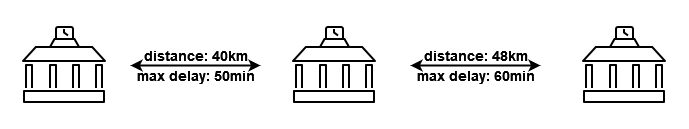
\includegraphics[scale=0.4]{images/poweredRailway.png}
\end{figure}
\bigskip

The second configuration doesn't verify the mandatory properties of the project and it is set as follows:
\\
\begin{figure}[H]
    \centering
    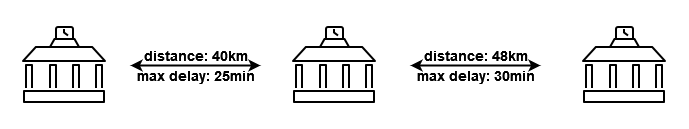
\includegraphics[scale=0.4]{images/poweredRailwaySimple.png}
\end{figure}
\bigskip

\subsection{Initializations}
The stations have the following initial configurations:
\begin{itemize}
    \item \textbf{Station 0: } 2 tracks, 1 available
    \item \textbf{Station 1: } 3 tracks, 2 available
    \item \textbf{Station 2: } 2 tracks, 0 available
\end{itemize}
\newpage

The trains that we designed have constant speed set to 120km/h. They are initialized as follows:
\begin{itemize}
    \item \textbf{Train 0 - charge 100: } starts from station 0 with station 2 as destination
    \item \textbf{Train 1 - charge 100: } starts from station 1 with station 2 as destination
    \item \textbf{Train 2 - charge 100: } starts from station 2 with station 0 as destination
    \item \textbf{Train 3 - charge 100: } starts from station 2 with station 0 as destination
\end{itemize}
\bigskip

\subsection{Design assumptions}
In order to efficiently describe the model, we decided to set a railway in which every station has less tracks than the total
number of train train, in order to obtain much more often situations in which a train has to wait to have the permission to enter
his next station.\\
Furthermore we decided not to design the railway with a dedicated template. That's because the railway's most important features are
implicitly designed and verified, without creating additional variables.\\
In the end, another assumptions that we made to simplify the description is that we assumed the clock unit as a minute.
